\documentclass[10pt]{article}
\usepackage{amsthm}
\usepackage{amsfonts}
%\usepackage{amsmath}
\usepackage[utf8]{inputenc}
\usepackage{graphicx}
\usepackage{xcolor}
\usepackage[margin=1.0in]{geometry}
\usepackage{fancyvrb}
\usepackage{cprotect}
\usepackage{url}
\usepackage{etoolbox}
\usepackage[hidelinks]{hyperref}
\usepackage[skins,theorems]{tcolorbox}
\usepackage{enumitem}
\usepackage{xcolor}
\usepackage{pifont}
\usepackage{tcolorbox}        % load once, no options
\tcbuselibrary{theorems,skins,breakable} % add features here
%\newcommand*{\vertbar}{\rule[-1ex]{0.5pt}{2.5ex}}
%\newcommand*{\horzbar}{\rule[.5ex]{2.5ex}{0.5pt}}
%\setlist[itemize]{align=parleft,left=1pt..1em}
% \usepackage{tikz}
% \usetikzlibrary{arrows.meta,positioning}
\newcommand{\vertbar}{\,\big|\,}

\usepackage{imakeidx}
\makeindex

\usepackage{listings}
\usepackage{xcolor}

% Define some colors
\definecolor{codegreen}{rgb}{0,0.6,0}
\definecolor{codegray}{rgb}{0.5,0.5,0.5}
\definecolor{codepurple}{rgb}{0.58,0,0.82}
\definecolor{backcolour}{rgb}{0.95,0.95,0.92}

% Define a style
\lstdefinestyle{mystyle}{
    commentstyle=\color{codegreen},
    keywordstyle=\color{blue},
    numberstyle=\tiny\color{codegray},
    stringstyle=\color{codepurple},
    basicstyle=\ttfamily,
    breakatwhitespace=false,
    breaklines=true,
    captionpos=b,
    keepspaces=true,
    numbersep=5pt,
    showspaces=false,
    showstringspaces=false,
    showtabs=false,
    tabsize=4
}

\lstset{style=mystyle}
%\usepackage[T1]{fontenc}
%\usepackage{inconsolata} % optional, nicer monospace font


\usepackage{cmbright}
%\usepackage[OT1]{fontenc}
%\usepackage{helvet}
%\renewcommand{\familydefault}{\sfdefault}

%\usepackage{titlesec}



%\titleformat{\section}
%  {\normalfont\fontsize{14}{17}\sffamily\bfseries}
%  {\thesection}
%  {1em}
%  {}
%
%\titleformat{\subsection}
%  {\normalfont\fontsize{12}{17}\sffamily\slshape}
%  {\thesubsection}
%  {1em}
%  {}



% from https://www.pinterest.co.uk/pin/88664686405122253/
\definecolor{C1}{RGB}{141, 125, 158} %purple
\definecolor{C2}{RGB}{163,156,147} % yellow
\definecolor{C3}{RGB}{99,151,153} % green
\definecolor{C4}{RGB}{195,106,99} % red
\definecolor{C5}{RGB}{124, 132, 128}
\definecolor{C6}{RGB}{67, 69, 75}



\definecolor{Gr}{HTML}{377D71}
\definecolor{Pu}{HTML}{A459D1}
\definecolor{Bl}{HTML}{4D455D}
\definecolor{Te}{HTML}{C1ECE4}
\definecolor{Or}{HTML}{EF6262}
\definecolor{Am}{HTML}{F3AA60}
\definecolor{Co}{HTML}{3C486B}
\definecolor{Wh}{HTML}{FEFBF6}
\definecolor{Ye}{HTML}{FFE196}
\definecolor{Re}{HTML}{E96479}
\definecolor{Pi}{HTML}{FFD0D0}
\definecolor{Rp}{HTML}{FF9EAA}
\definecolor{Wg}{HTML}{EEF3D2}

\newcounter{unit}
\renewcommand{\thesection}{\theunit.\arabic{section}}

\hypersetup{
    colorlinks=false,
    linkcolor=red,
    filecolor=red,      
    urlcolor=red,
    pdftitle={a},
    pdfpagemode=FullScreen,
    }
    
    
 % TCOLORBOX STUFF ----------------------------------------------------------------------------
 

 %  ----------------------------------------------------------------------------
    
%\patchcmd{\section}{\normalfont}{\color{C5}}{}{}
%\patchcmd{\subsection}{\normalfont}{\color{C5}}{}{}


\newcommand{\dfn}[1]{{\underline{#1}}}
\definecolor{sidebarblue}{HTML}{E3F2FD}


\renewcommand{\FancyVerbFormatLine}[1]{\color{gray}{>\,\,#1}}
    
\newtheorem{thm}{Theorem}


\newtheoremstyle{exercise}
{}                % Space above
{}                % Space below
{\color{black}}        % Theorem body font % (default is "\upshape")
{}                % Indent amount
{\bfseries}       % Theorem head font % (default is \mdseries)
{:}               % Punctuation after theorem head % default: no punctuation
{ }               % Space after theorem head
{}                % Theorem head spec
\theoremstyle{exercise}
\newtheorem{exercise}{Exercise}


\newtheoremstyle{example}
  {}                % Space above
  {}                % Space below
  {\color{black}} % Theorem body font (default is "\upshape")
  {}                % Indent amount
  {\bfseries}       % Theorem head font (default is \mdseries)
  {.}               % Punctuation after theorem head (default is no punctuation)
  { }               % Space after theorem head
  {\thmname{#1}\thmnumber{ #2}\thmnote{ \textnormal{(#3)}}}  % Theorem head spec: #1 is name, #2 is number, #3 is note

\theoremstyle{example}
\newtheorem{example}{Example}

% Boxed, breakable 'example' with dashed continuation markers and custom background
	\tcolorboxenvironment{example}{
  enhanced,
  breakable,
  colback=sidebarblue,        % <<< background color
  colframe=black,
  boxrule=1pt,
  arc=5pt,
  left=6pt,right=6pt,top=6pt,bottom=6pt,
  % dashed markers at page breaks
  overlay unbroken={},   % no markers if the box doesn't break
 }

\newtheoremstyle{solution}
{}                % Space above
{}                % Space below
{\color{C5}}        % Theorem body font % (default is "\upshape")
{}                % Indent amount
{\bfseries }       % Theorem head font % (default is \mdseries)
{:}               % Punctuation after theorem head % default: no punctuation
{\newline}               % Space after theorem head
{}                % Theorem head spec
\theoremstyle{solution}
\newtheorem*{solution}{Solution}


\newcommand{\mcS}{\mathcal S}
\newcommand{\mcR}{\mathcal R}
\newcommand{\mcC}{\mathcal C}
\newcommand{\bS}{{\boldsymbol S}}
\newcommand{\bR}{{\boldsymbol R}}
\newcommand{\bC}{{\boldsymbol C}}
\newcommand{\ba}{{\boldsymbol a}}
\newcommand{\bb}{{\boldsymbol b}}
\newcommand{\bs}{{\boldsymbol s}}
\newcommand{\bff}{{\boldsymbol f}}
\newcommand{\br}{{\boldsymbol r}}
\newcommand{\bx}{{\boldsymbol x}}
\newcommand{\bt}{{\boldsymbol t}}
\newcommand{\bv}{{\boldsymbol v}}
\newcommand{\bu}{{\boldsymbol u}}
\newcommand{\bw}{{\boldsymbol w}}
\newcommand{\bc}{{\boldsymbol c}}
\newcommand{\be}{{\boldsymbol e}}
\newcommand{\bq}{{\boldsymbol q}}
\newcommand{\bphi}{{\boldsymbol \phi}}
\newcommand{\brho}{{\boldsymbol \rho}}
\newcommand{\btau}{{\boldsymbol \tau}}
\newcommand{\reals}{\mathbb R}
\newcommand{\ints}{\mathbb N}
\newcommand{\E}{\mathbb E}
\newcommand{\Prob}{\mathbb P}


\newcommand{\sectionrefs}[1]{\par\smallskip\noindent\textbf{References:} #1\par\smallskip}


%%%%%%%%%%%%%%%
% adding space between items
%\usepackage{enumitem}
%\setlist{topsep=1.5em, itemsep=1.1em}





\setcounter{unit}{1}
\setcounter{section}{0}

\begin{document}



\title{Unit 5: Beyond strict linearity}
\author{Ethan Levien}
\maketitle
\tableofcontents
%----------------------------------------------------------------------------------------------------------------
%\section{Reading}
%\begin{itemize}
%\item  \cite[Section 10.1]{islp}
%\begin{itemize}
%\item Example 10.1.2. This is the linear regression model with multiple predictors. 
%\item This entire section is useful and all the exercises are good practice. 
%\end{itemize}
%\item \cite[Section 10.2]{tabak}
%\item \cite[Section 10.5]{tabak}
%\item \cite[Section 3.2]{islp}
%\end{itemize}




\section{Interactions}


The important assumption of the multiple predictor regression models we have seen so far is that the ``effect'' of one predictor does not depend on the value of the other. Here are some examples where this could be violated:
\begin{itemize}
\item The difference in test scores between kids whose mothers did and and did not go to high school depends on their mother's score on the iq test.
\item  The association between earnings and height depends on gender, e.g. being taller tends to give men a larger advantage than women
\item The effect of a drug for treating covid depends on whether someone has had covid before. 
\end{itemize}
We call the dependencies described above \dfn{interactions}. 
It turns out it is possible to include interactions within the regression modeling framework we have already introduced, as is illustrated by the following example. 
 Let's work in the case of two predictors. If you'd like, you can refer to Example \ref{ex:testscores} to make this math more concrete and always replace $X_1$ with $X_{\rm hs}$ and $X_2$ with $X_{\rm iq}$.   In each of the cases above, what is going on is that the slope of $\E[Y|X_1,X_2]$ vs. $X_1$ for fixed $X_2$ is not a constant, $\beta_1$, but rather something that depends on $X_2$. The simplest way to account for this is to let effect of $X_2$ on the slope be linear in $X_2$, so instead of $\beta_1$ being the slope of $\E[Y|X_1,X_2]$ vs. $X_1$ we would have $\beta_1 + \beta_{1,2}X_2$ be this slope, but this leads to a regression model with a nonlinear term: 
\begin{equation*}
Y = \beta_0 +(\beta_1 + \beta_{1,2}X_2) X_1  + \beta_2 X_2 = \beta_0 + \beta_1 X_1 + \beta_2 X_2 + \beta_{1,2}X_1 X_2 + \epsilon 
\end{equation*}
We call $X_1X_2$ an \dfn{interaction} term, but Yuck! This isn't linear anymore and the regression coefficients are also don't have the same interpretation. How do we deal with this? 
 The idea is that we can create a new predictor from our already existing predictors which accounts for the interactions. To this end, consider the two predictor regression model written now as 
\begin{equation*}
Y = \beta_0' + \beta_1' X_1 + \beta_2' X_2 + \epsilon.
\end{equation*} 
I'm again using the $'$ to distinguish this model from an expanded model with a new predictor. The new predictor which accounts for the interaction will be $X_3 = X_1X_2$! Note that $X_3$ is going to be correlated with both $X_1$ and $X_2$, but crucially it will not be perfectly correlated unless $X_1$ and $X_2$ are with each other. The new mode is 
\begin{equation*}
Y = \beta_0 + \beta_1 X_1 + \beta_2 X_2 + \beta_{1,2}X_3 + \epsilon
\end{equation*} 
Or written as a conditional distribution 
\begin{equation*}
Y|X \sim {\rm Normal}( \beta_0 + \beta_1 X_1 + \beta_2 X_2 + \beta_{1,2} X_3, \sigma^2). 
\end{equation*} 
 Now how do we interpret the regression coefficients in the new model? 
If we write out the usual formula for the regression coefficient with no interactions, we get 
\begin{align*}
 &\E[Y|X_1 = x+1,X_2] -\E[Y|X_1 = x,X_2]\\
 &  =  \left(\beta_1 (x+1)+ \beta_2 X_2 + \beta_3 (x+1)X_2\right)- \left(\beta_1 x + \beta_2 X_2 + \beta_{1,2} x X_2\right)\\
 &= \beta_1 + \beta_{1,2}X_2
\end{align*}
Here I've replaced $X_3$ with $X_1X_2$. I words, $\beta_{1,2}$ is the additional difference in the regression slope between $Y$ and $X_1$ with all other predictors fixed when $X_2$ is changed by one unit. 
If $\beta_{1,2}$ is positive (resp. negative) then increasing $X_2$ has a tendency to increase (resp. decrease) the difference between the conditional averages of $Y$, thus, the additional predictor $X_3 = X_1X_2$ allows us to capture an interaction wherein the association between $X_1$ and $Y$ depends on $X_2$. We can do the same calculation with $X_1$ fixed and $X_2$ changed to obtain 
\begin{equation*}
 \E[Y|X_1 = x+1,X_2] - \E[Y|X_1 = x,X_2] = \beta_2 + \beta_3X_2
\end{equation*}
Now as always, let's make sure we understand how this translates into code and also I think the visualizations in this example are helpful. 


\begin{example}[Visualizing interactions]
Consider the regression model with interactions term $X_3 = X_1X_2$ defined above, assuming that 
\begin{align*}
X_1 &\sim {\rm Normal}(0,1)\\
X_2 &\sim {\rm Bernoulli}(1/2)
\end{align*}
Assume $\beta_1 = 1.2,\beta_2 = 0$ and $\beta_3 =-1$. \\


\noindent
\underline{Question:} What are the slopes of $E[Y|X_1,X_2=0]$ vs. $X_1$ and $E[Y|X_1,X_2=1]$ vs. $X_1$? Plot these in colab. 


\end{example}

\begin{example}[Interaction in test score model]\label{ex:testscores}
Here we once again consider the test score data with high school education and IQ as predictors. In particular, we will fit the model
\begin{equation*}
Y = \beta_0 + \beta_{\rm hs}X_{\rm hs} + \beta_{\rm iq}X_{\rm iq} + \beta_{\rm iq,hs}X_{\rm iq}X_{\rm hs}
\end{equation*}


\noindent
\underline{Question:} 
\begin{enumerate}[label=(\alph*)]
%\item Is there a statistically significant ($p_v<0.05$) interaction between high school and IQ? 
\item What are the values and interpretations of the regression coefficients in the new model?
\item What do the results tell us about the ``effect'' of IQ on test scores and how it is related to high school education? \\
\end{enumerate}

\noindent
\underline{Solutions:} 
The output of \verb!statsmodels! is 
\begin{Verbatim}
==============================================================================
                 coef    std err          t      P>|t|      [0.025      0.975]
------------------------------------------------------------------------------
const        -11.4820     13.758     -0.835      0.404     -38.523      15.559
mom_hs        51.2682     15.338      3.343      0.001      21.122      81.414
mom_iq         0.9689      0.148      6.531      0.000       0.677       1.260
hs_iq         -0.4843      0.162     -2.985      0.003      -0.803      -0.165
\end{Verbatim}
\vspace{.4cm}

\begin{enumerate}[label=(\alph*)]
%\item There statistically significant interaction effect since the $p$-value of the interaction coefficient is $0.003$. 
\item The values and interpretations are as follows
\begin{itemize}
\item $\beta_0 \approx -11$ does not have a clear interpretation since it doesn't make sense to have $0$ IQ. 
\item $\beta_{\rm iq}\approx 1$ is the expected signed difference in scores between students whose IQ differs by $1$ point and whose mothers did not go to high school. 
\item $\beta_{\rm hs} \approx 51$ is the expected difference between scores of students whose mothers did and did not go to high school when IQ is zero -- {\bf much like $\beta_0$, this doesn't really make sense, so we don't have a clear interpretation of $\beta_{\rm hs}$}
\item $\beta_{\rm hs,iq}\approx -0.5$ is the expected increase between the group of students whose mothers attended high school and those that did not in the difference between test scores of students whose mothers iq differs by one point. In other words, it is the increase in regression slope of scores vs. iq between the two high school groups. It is easier to interpret $\beta_{\rm iq}  + \beta_{\rm hs,iq}$ which is the expected signed difference in scores between students whose IQ differs by $1$ point and whose mothers did attend high school (this is the same as the interpretation of $\beta_{\rm iq}$ for student's whose mothers attended high school. 
\item It appears that the association between IQ and test scores is weaker among students whose mother's attended high school. This makes intuitive sense. If someone attended high school the subtle differences in cognitive ability that IQ is supposed to measure are not as relevant. 
\end{itemize}
\end{enumerate}



\end{example}

In the example above we saw that adding an interaction term can make the interpretation  of the regression coefficients a bit clunky, even those regression coefficients that are not involved in an interaction. In particular, we ran into the problem that the interpretation of $\beta_{\rm iq}$ was lost. To remedy this, we can define the centered predictor
\begin{equation*}
\Delta_{\rm iq} = X_{\rm iq} - \bar{X}_{\rm iq} 
\end{equation*}
and now we fit the model 
\begin{equation*}
Y =  \beta_0 +  \beta_{\rm hs} X_{\rm hs} + \beta_{\rm iq}\Delta_{\rm iq} +  \beta_{\rm hs-iq}X_{\rm hs}\Delta_{\rm iq} + \epsilon 
\end{equation*}
Now $\beta_1$ has the interpretation as the average difference in scores among students whose mothers have the average iq. You can also standardize the predictor to get around the awkward interpretation of the regression coefficients. 






%----------------------------------------------------------------------------------------------------------------
\subsection{Residual plots (Optional)}


 We address the question of how we might identify when it is appropriate to add an interaction term to a model. In this case of two predictors we can easily visualize the data by making plots of the $Y$ vs. $X_1$ slopes for different $X_2$ values (especially  when one predictor is binary). With many predictors, it becomes less clear what plot might reveal some hidden interaction terms. We could of course go on adding every possible interaction term, but with many predictors this becomes in practical and leads to overfitting (as we will soon discuss). 
 The basic idea of \dfn{residual  plots} is that by plotting the difference between the observed $y$ values and the prediction of the $E[Y|X]$, or 
\begin{equation*}
\epsilon_j  = Y_j - \hat{\beta}_0 - \sum_k^{K}\hat{\beta}_kX_{k,j}
\end{equation*}
where $X_{k,j}$ is the value of predictor $i$ at the $j$th data point. 
Our goal is to plot $\epsilon_j$ in a such a way that disagreement between our model and the data is revealed by this plot.  In the instance of a single-predictor, we can simply plot $\epsilon_j$ as a function of the predictor $X$. If we notice that the residuals do not appear to follow a normal distribution, or that the variance and mean change, then we should be skeptical.
 The question is: {\bf When we have multiple predictors, what do we plot on the horizontal axis?}   The answer is to plot $\epsilon_j$ as a function of the predictors value of $E[Y|X]$; that is $\epsilon_j$ vs. $\hat{y}_j = \sum_i^{K} \hat{\beta}_iX_{i,j}$. The following examples is supposed to help us understand why. 




\begin{figure}[h]
    \centering
    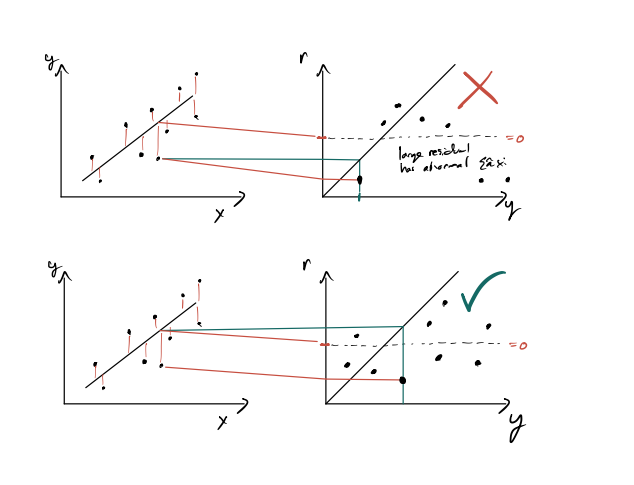
\includegraphics[width=0.8\textwidth]{./../figures/res}
    \caption{Correct and incorrect way to plot residuals against response variable }
    \label{fig:res}
\end{figure}

\begin{example}[Residual plots]\label{ex:res}

Consider the regression model with two predictors and suppose the true parameter values are $\beta_0=0$,$\beta_1 = 0.2$,$\beta_2 = 20$ and $\sigma = 1$. \\


\noindent
\underline{Question:} Compare two ways of plotting the residuals 
\begin{enumerate}[label=(\alph*)]
\item Plot $\epsilon_i$ as a function of $\sum_k^{K}\hat{\beta}_kX_{k,i}$. 
\item Plot $\epsilon_i$ as a function of $Y_i$. Why does there appear to be a bias towards high values of $\epsilon_i$ for large $Y_i$ that is not present in the first plot? \\
\end{enumerate}


\noindent
\underline{Solution:} See \href{https://colab.research.google.com/drive/1UTUUfWTpmazSa40sqLUWAojRi2kGJM-O?usp=sharing}{colab notebook}

\end{example}

 To better understand what the residual plot tells us, recall
\begin{equation}\label{eq:resapprox}
\epsilon_j \approx Y_j - \underbrace{E[Y|(X_1,\dots,X_K) = (X_{1,j},\dots,X_{K,j})] }_{\approx \hat{\beta}_0 + \sum_k^{K}\hat{\beta}_kX_{k,j}}
\end{equation}
where $K$ is the number of predictors. 
Thus, the distribution of $\epsilon_j$ is approximately 
\begin{equation*}
\epsilon_j \sim {\rm Normal}(0,\sigma^2). 
\end{equation*}
This tells us how the points should be distributed in the vertical direction. It {\bf does not} say anything about the distribution of points in the horizontal direction, which is determined by the distribution of the predictors. Therefore, we expect a plot which is symmetric around the line $\epsilon_j$ for all values of $\hat{y}_j$ (our predicted values of $Y$), but any distribution in the horizontal direction is okay. 

Now compare this to what would happen if we plotted $Y_j$ on the horizontal axis, not $\hat{y}_j$. In this case, based on Equation \ref{eq:resapprox} $\epsilon_j$ and $Y_j$ are correlated. This is why we see a bias of the residuals for small/large $Y_j$ in Example \ref{ex:res}. 






%----------------------------------------------------------------------------------------------------------------
\section{Other nonlinear models}

 Here, we discuss how to build more complex models and directly access their predictive power on out-of-sample data.  %Previously, we saw that we can indirectly access it by looking at model assumptions and $R^2$
In the context of interactions, we already saw saw how a model can be extended by defining a new predictor $X_3 = X_1X_2$. The more general idea that we can define a new predictor which is a function of the other predictors allows us to develop very complex and flexible models which nonetheless can be analyzed within linear regression framework. Here, we will formalize this, beginning with the case of a single predictor. 

In general, the linear regression framework allows us to fit models of the form consider the model
\begin{equation}\label{eq:nlgauss}
Y|X \sim {\rm Normal}( f(X),\sigma^2)
\end{equation}
provided we can express $f(X)$ as a linear combinations of nonlinear functions of $X$. What I mean by this is that we can find function $\phi_1(x),\dots,\phi_K(x)$ such that 
\begin{equation*}
f(X) = \sum_{i=1}^K \beta_i\phi_i(X)
\end{equation*}
The functions $\phi_i(X)$ are often referred to as \dfn{basis functions}, or \dfn{features} in machine learning lingo. We can think of each $\phi_i(X)$ as a new predictor. 



\begin{example}[Simulating a nonlinear model]

Consider the conditional Gaussian model given in Equation \ref{eq:nlgauss} with 
\begin{equation*}
f(x) = \beta_0+\beta_1x + \beta_2x^2
\end{equation*}
 This is simply a linear model once we define the new predictors 
\begin{align*}
X_1 &= \phi_1(X) = X\\
X_2 &= \phi_2(X) = X^2. 
\end{align*}


\noindent
\underline{Question:}
\begin{enumerate}[label=(\alph*)]
\item Generate data from this model
\item Fit the data to the model using \verb!statsmodels!.\\
\end{enumerate}

\noindent
\underline{Solution:}
See \href{https://colab.research.google.com/drive/1q3mfX4od6iLFHy2dYFaKzw6FjaTbAaD3?usp=sharing}{colab notebook}

\end{example}



\begin{figure}[h]
    \centering
    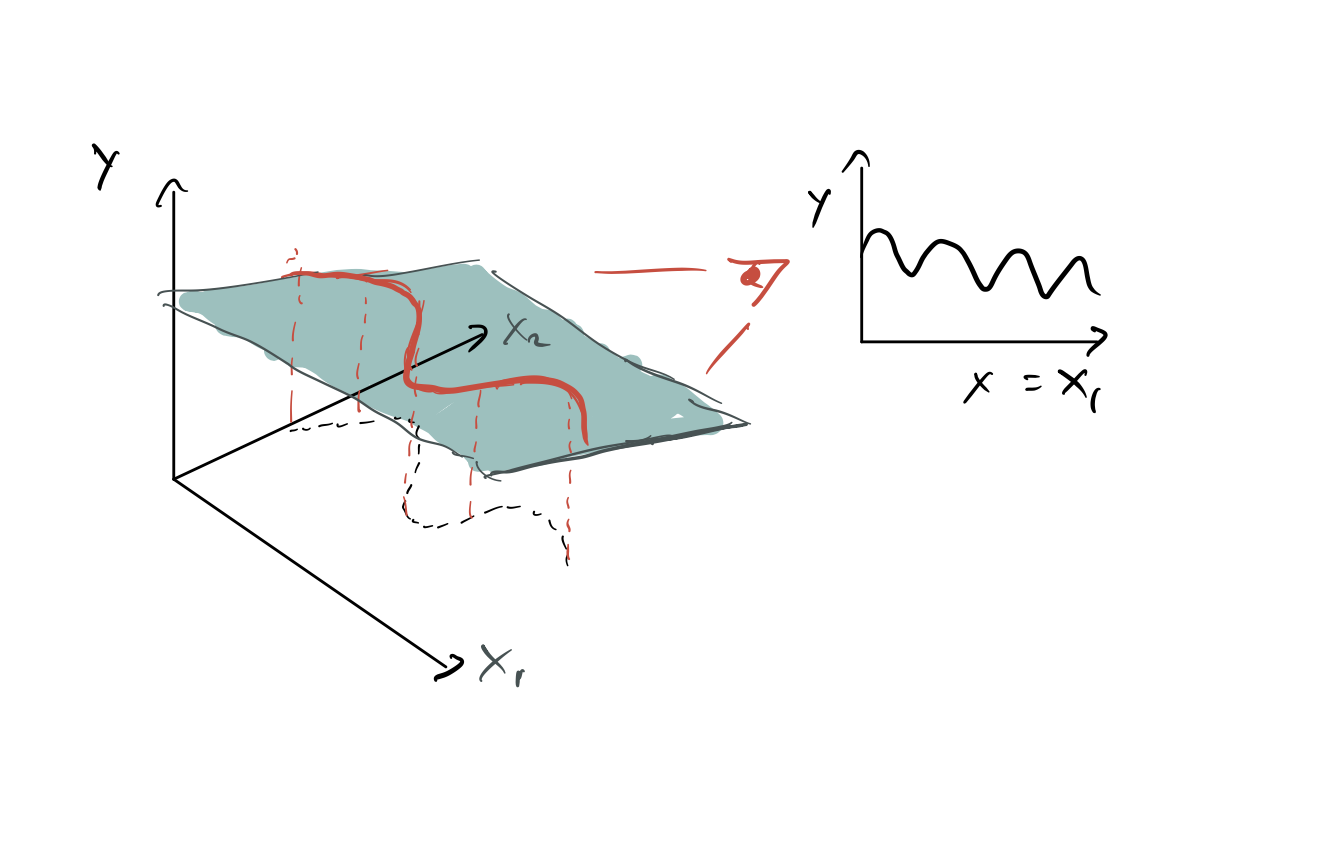
\includegraphics[width=0.8\textwidth]{./../figures/feature}
    \caption{An illustration of how a nonlinear dependence on our predictor can be incorporated into the linear modeling framework by adding a feature.}
    \label{fig:feature}
\end{figure}

Which functions $\phi$ should we use? The answer of course depends on the problem at hand. For example, we might know something about the physics of the data we are modeling. In some cases, we may select the $\phi$ so that the parameters $a_i$ have clear interpretations (as is the case in linear regression model). The following illustrates such an example.  

\begin{example}[Mauna Kea Data]

\noindent
\underline{Solution:} See \href{https://colab.research.google.com/drive/1q3mfX4od6iLFHy2dYFaKzw6FjaTbAaD3?usp=sharing}{colab notebook}


\end{example}

Next we will  understand that within the linear regression framework we can fit very complicated nonlinear data. However, we need to be careful when adding new features to the model. The following example will illustrate how it is possible to ``overshoot'' and make our too complex. In the next set of notes we will dive much deeper into this, bridging the gap between machine learning and statistics. 


%----------------------------------------------------------------------------------------------------------------
\section{Cross validation}

We saw from the previous example that $R^2$ is not very helpful if we want to decide how complex we'd like to make our model, since it is possible to explain all the variation in the $Y$ values with a model which is too complex. In order to address this, we take the approach of \dfn{cross validation}. The basic idea of cross validation is to break our data up into two subsets: \dfn{training set}, which we use to fit the model, and a \dfn{testing set}, which we compare to the predictions of the fitted model. 
 {\bf Some Notation}

 I will use $D$ to refer to our entire data set:
\begin{equation*}
D = (Y,X) = \{(X_1,Y_1),\dots,(X_N,Y_N)\}
\end{equation*}
 $D^{\rm train} = (Y^{\rm train},X^{\rm train})$ and $D^{\rm test} = (Y^{\rm test},X^{\rm test})$ will represent the subsets of the data to be used to training (that is, fitting) the model and testing the fit respectively.  We will assume that
\begin{equation*}
D = D^{\rm train} \cup D^{\rm test}
\end{equation*}
 Let $N_{\rm train}$ and $N_{\rm test}$ denote the number of points in each group.
 Let $\hat{y}(x,D)$ the prediction of $E[Y|X =x]$ using the fitted coefficients based on a data set $D$; that is
\begin{equation*}
\hat{y}(x,D) = \sum_{i=1}^{K}\hat{\beta}_i\phi_i(x)
\end{equation*} 
where $\hat{\beta}$ are the (usually least squares) fitted coefficients using the data in $D$. 




Now let us define the \dfn{training error}
\begin{equation*}
\epsilon_{\rm train}^2=  \frac{1}{N_{\rm train}}\sum_{i=1}^{N_{\rm train}}(\hat{y}(X_i^{\rm train},D^{\rm train}) - Y_i^{\rm train})^2
\end{equation*}
where the average is taken over different replicates of our data and $\hat{Y}_i$ is our prediction of $E[Y|X]$. Not that the training error tells us about how well our model does at predicting the same data we used to fit it, and therefore not surpisingly, it is closely related to $R^2$:
\begin{equation*}
R^2 \approx 1 - \frac{\epsilon_{\rm train}^2}{{\rm var}(Y_{{\rm train},i})}.
\end{equation*}

In order to see how well our model does at predicting the points we did NOT use to fit it, we introduce the test error: 
\begin{equation*}
\epsilon_{\rm test}^2=  \frac{1}{N_{\rm test}}\sum_{i=1}^{N_{\rm test}}(\hat{y}(X_i^{\rm test},D^{\rm train}) - Y_i^{\rm test})^2
\end{equation*}
Note that the fitted coefficients used to compute $\hat{y}_i(X^{\rm test})$ come from fitting the model to the training data, even though we are evaluating $\hat{y}$ at the test points. 

\begin{example}[Cross validation on polynomial model]\label{ex:polycrossval}
Consider example 6 from the previous weeks notes. \\

\noindent
\underline{Question:} Plot the training and test error as a function of the number of parameters. \\

\noindent
\underline{Solution:}  See \href{https://colab.research.google.com/drive/1EYcMviowfsnsVe7vsUKlyzkNsddUiTau?usp=sharing}{colab notebook}.
\end{example}

%----------------------------------------------------------------------------------------------------------------
\section{Bias, variance and overfitting}
 In order to understand U-shaped curve seen in Example \ref{ex:polycrossval},  we first need to introduce some more general terminology and notation for talking about estimators (of which $\hat{y}$ is an example). 
To this end, we introduce the \dfn{mean-squared error} of an estimator $\hat{\theta}$ of some quantity $\theta$. $\theta$ could be a parameter, or it could be a value of a function, such as $f(x)$, that we would like to predict. 
\begin{equation}\label{eq:mse}
{\rm MSE}_{\hat{\theta}}= E\left[(\hat{\theta}- \theta)^2\right]
\end{equation}
 For now, let's just think of $\hat{\theta}$ as any estimator. 
 The following theorem is the key result which will allow us to understand the U-shaped curve. 
\begin{thm}[Bias variance decomposition]
\begin{equation}\label{eq:biasvar}
{\rm MSE}_{\hat{\theta}} = {\rm var}(\hat{\theta}) + E\left[\hat{\theta}-\theta\right]^2
\end{equation}
\end{thm}
\begin{proof}
Using the definition of variance 
\begin{equation*}
{\rm var}\left(\hat{\theta}-\theta\right) = E\left[(\hat{\theta}-\theta)^2\right] - E\left[\hat{\theta}-\theta\right]^2. 
\end{equation*}
Since $\theta$ is a constant, ${\rm var}\left(\hat{\theta}-\theta\right)= {\rm var}\left(\hat{\theta}\right)$, so 
rearranging terms yields the result. 
\end{proof}
Now let's break this result down a bit. 


 The first term in Equation \ref{eq:biasvar} is simply the variance, which in the case of an estimator of a parameter we can recognize as the squared standard error. This is tell us how much variation there is in our estimate from replicate of replicate. You should recognize that a consistent estimator is exactly one for which this quantity vanishes when $N$ is very large. 
 The second term is what we will define as the squared of the bias: 
\begin{equation*}
{\rm Bias}_{\hat{\theta}} = E[\hat{\theta}-\theta].
\end{equation*}
This tell us whether our estimate will on average give us the correct value of $\theta$. You should recognize that an unbiased estimator is exactly one for which this quantity is zero!

 Now let's return to working in the context of a model of the form 
\begin{equation*}
Y|X \sim {\rm Normal}(f(X),\sigma^2)
\end{equation*}
where $f(X)$ can be written as a linear combination of features
\begin{equation*}
f(X) = \sum_{i=1}^N\beta_i \phi_i(X). 
\end{equation*}
Letting $\hat{\theta} = \hat{y}(x,D)$, applying Equation \ref{eq:mse} yields
\begin{equation*}
{\rm MSE}_{\hat{y}(x,D)} = E\left[(\hat{y}(x,D)- f(x))^2\right]
\end{equation*}
where the average is taken over replicates of our data $D$. This is a measurement of our ability to predict $f(x)$, which is exactly what the test error seeks to measure. 
  To more closely relate the bias-variance tradeoff to the test error, we will use a slightly different definition of MSE, which is 
\begin{equation}\label{eq:tilMSE}
\widetilde{{\rm MSE}}_{\hat{y}(x,D)} = E\left[(\hat{y}(x,D)- Y(x))^2\right]
\end{equation}
where $Y$ is a sample from $Y|(X=x)$. You can show (see Exercise) that
\begin{equation*}
\widetilde{{\rm MSE}}_{\hat{y}(x,D)} = \sigma^2 +{\rm var}(\hat{y}(x,D)) + E\left[\hat{y}(x,D)-f(x)\right]^2
\end{equation*}
The new term, $\sigma^2$, captures the fact that, unlike the deterministic term $f$, we can NEVER predict the \emph{random} variable $Y$ exactly. 
You should be able to justify that
\begin{equation*}
\epsilon_{\rm test}^2 \approx E\left[\widetilde{{\rm MSE}}_{\hat{y}(X,D^{\rm train})}\right]
\end{equation*}
 The important thing to recognize is that a complicated model will tend to have a higher variance, since it will be able to change more in response to data. Meanwhile, a very simple model will tend to have a higher bias. 



\begin{example}[Plotting Bias and variance]

Let's continue with Example \ref{ex:polycrossval} and try to illustrate the bias variance tradeoff by computing these (or really approximations to them) separately. \\


\noindent
\underline{Solution:}  See \href{https://colab.research.google.com/drive/1EYcMviowfsnsVe7vsUKlyzkNsddUiTau?usp=sharing}{colab notebook}.

\end{example}

 We now summarize some observations we've made thus far:
\begin{itemize}
\item In a regression model, as we add more coefficients, eventually the model becomes more and more ``flexible'', in the sense that is can describe more different types of data sets. Here, by ``describe'', we mean that it can be fit to those data sets with a small value of $R^2$ or training error.  With enough features, a model can perfectly interpolate between the data points, meaning $\hat{y}(X_i,D) = Y_i$ for each data point $(X_i,Y_i)$ when the model is fit on all our data points. 
\item Unlike the training error and $R^2$, the test error, $\epsilon_{\rm test}^2$ does not simply increase as we make the model more complex, rather it has a U-shape. Thus, there is a optimal model size at which our model's predictions of new data points -- that is, data points outside the set we used to fit it -- is best. 
\item The $U$-shape can be understood in terms of bias and variance. We know this because the mean-squared error, which is the ``math world'' version of $\epsilon_{\rm test}^2$, can be decomposed into a bias and variance term. The variance term tells us how variable the predictions of our model will be when we fit it to different training sets, while the bias tells us how much its predictions. will differ, on average, from real data. 
\end{itemize}

\begin{figure}[h]
    \centering
    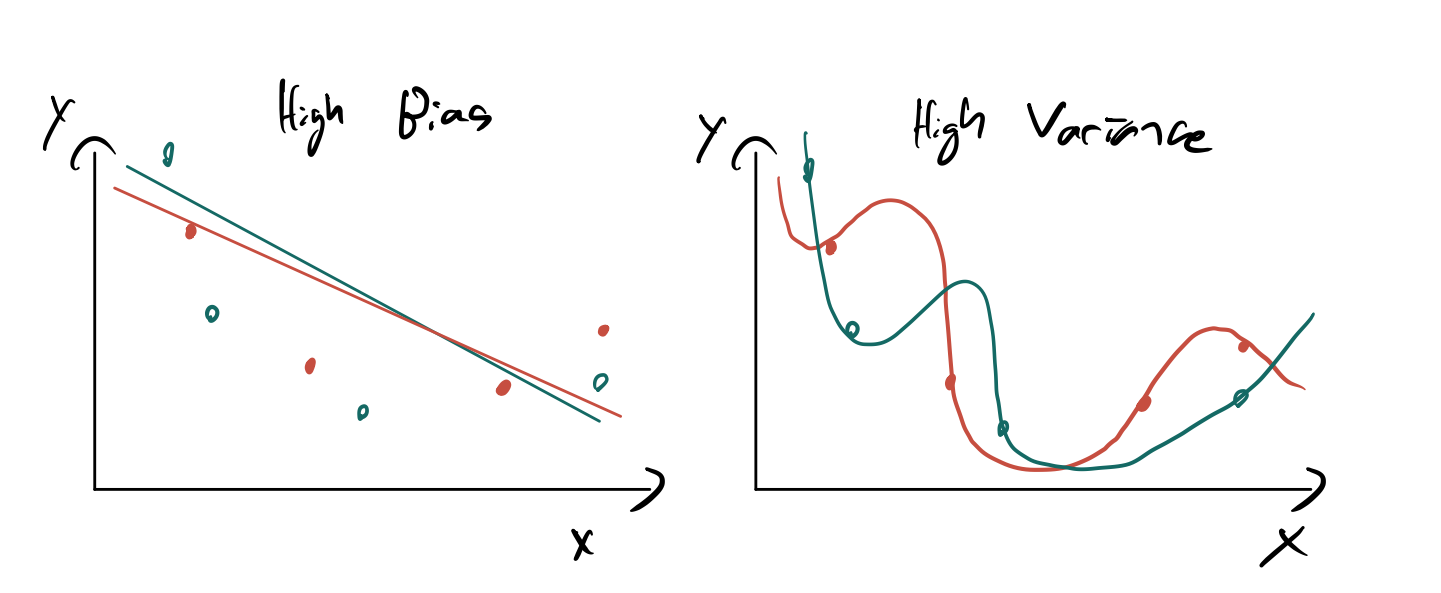
\includegraphics[width=0.8\textwidth]{./../figures/bias_var}
    \caption{Bias and variance illustrated with fits to two different datasets (blue and red) drawn the from the same distribution}
    \label{fig:bv}
\end{figure}







\section{Orthogonality and Fourier analysis (optional)}
 Sometimes we have a particularly hypothesis about what features my contribute to an signal we are analyzing -- for example, the CO2 data from last week we suspected there was a linear trend and yearly trend superimpose together. This was reasonable because we know that whether tends to follow a yearly cycle. But in general, if we don't have such knowledge how should we select the functions $\phi$?  It is often to our advantage to select basis function $\phi_i$ so that our predictors are not correlated. That is, if $\phi_i(X)$ and $\phi_j(X)$ are thought of as random variables (the randomness comes from $X$) then we want them to be uncorrelated. 


Throughout our discussion, we will assume that $E[\phi_i(X)]=0$. We can easily make this so by subtracting the means of our features. Therefore, we would like to find $\phi_i$ such that 
\begin{equation}\label{eq:orth}
E[\phi_i(X)\phi_j(X)] = 0 \quad i\ne j.
\end{equation}
We this holds for some distribution of $X$, we say that $\phi_i$ and $\phi_j$ are \dfn{orthogonal} with respect to this distribution.



\begin{example}[Sin series]\label{ex:sin}

Let us now work with the particular example where 
\begin{equation}\label{eq:Xunif}
X \sim {\rm Uniform}(-L,L).
\end{equation}
Even if our $X$ points are not random, but are say evenly spaced on the interval $[-L,L]$, a random sample from the uniform distribution will be statistical similar to some randomly selected evenly spaced $X$ points. Thus, we can think of the uniform distribution as approximating the spread of our $X$ data with a random variable. 

Now consider the basis functions 
\begin{equation*}
\phi_j(x) = \sin\left(\frac{\pi x j}{L} \right).
\end{equation*}

 


\noindent
\underline{Question:} Show using simulations that $\phi_j$ are orthogonal with respect to the uniform distribution on $[-L,L]$ (Equation \ref{eq:Xunif}). \\


\noindent
\underline{Solution:}  See \href{https://colab.research.google.com/drive/1EYcMviowfsnsVe7vsUKlyzkNsddUiTau?usp=sharing}{colab notebook}.

\end{example}


Notice that if $\phi_j$ are orthogonal, then we can express the regression coefficients as
\begin{equation*}
\beta_j = \frac{{\rm cov}(Y,\phi_j(X))}{{\rm var}(\phi_j(X))} =  \frac{E[Y\phi_j(X)]}{E[\phi_j(X)^2]}
\end{equation*}
and hence our fitted coefficients from $N$ data points can be approximated as
\begin{equation}\label{eq:fourier_coef}
\hat{\beta}_j \approx \frac{\sum_{i=1}^N\phi_j(X_i)Y_i}{\sum_{i=1}^N\phi_j(X_i)^2}
\end{equation}
This suggests $\hat{\beta}_j$ should depend only weakly how many of the features $\phi$ we have included in our model! This is consequence of orthogonality. In contrast,  in the earlier example where we used polynomial features adding a new predictor, say $X^4$, would dramatically change the fitted value of $\beta_2$. However, 
Now let's return to Example \ref{ex:sin}. A limitation of this model is that it only permits us to model ``odd functions'' that is, functions for which $f(x) = -f(x)$, as each $\phi_j$ has this property. It is therefore desirable to add addition features which permit this, but we'd like them to still be orthogonal. To this end, we introduce a new set of features to the model given by the cosine functions:
\begin{equation*}
 \cos\left(\frac{\pi x j}{L} \right).
\end{equation*} 
Our new model, called a \dfn{Fourier series}, is given by 
\begin{equation*}
f(x) = \beta_0 + \sum_{i=1}^K\beta_i\sin\left(\frac{\pi i x }{L} \right) + \alpha_i \cos\left(\frac{\pi i x }{L} \right)
\end{equation*}
where we are using $\alpha_i$ to represent the coefficients of the cosine terms. Fourier series are on of the most important models in data science and engineering. It can be proved that as $K \to \infty$ we can approximate essentially ANY function with a series of this form.


\begin{example}[Working with Fourier series in python]\label{ex:fourier}
Suppose we have data from the model with 
\begin{equation*}
f(x) = \sin(3\pi x) + \sin (10\pi x)
\end{equation*}
where $X_i = (i-1)/N$ (meaning the $X$ points are evenly spaced in $[0,1]$. \\



\noindent
\underline{Question:} For different values of $\sigma^2$, generate data from this model and fit it to a Fourier series with $K=100$ terms. \\



\noindent
\underline{Solution:} See \href{https://colab.research.google.com/drive/1EYcMviowfsnsVe7vsUKlyzkNsddUiTau?usp=sharing}{colab notebook}. \\


\end{example} 

The process of computing the coefficients $\hat{\beta}_j$ and $\hat{\alpha}_j$ for the Fourier series is called  a \dfn{Discrete Fourier Transform}. Usually DFT refers to the cases where the $X_i$ are equally spaced. In this case, the orthogonality condition (Equation \ref{eq:orth}) is true is ``data world'', not just ``math word'' -- what I mean by this is that for equally spaced data points. 

To be precise, consider the predictor data on the interval $[0,L]$ given by 
\begin{equation*}
X_i = \frac{L(i-1)}{N-1}
\end{equation*}
for $i=1,\dots,N$. Thus $X_1 = 0$, $X_2 = L/N$, $X_3 = 2L/N$ and $X_N = L$. We could generate these points with \verb!np.linspace!. The following theorem tells us that the empirical, or sample covariance between the sin features, is exactly zero for these predictors.

\begin{thm}
\begin{equation*}
\sum_{i=1}^N\sin\left(\frac{2\pi j X_i}{L}\right) \sin\left(\frac{2\pi k X_i}{L}\right)  =0\quad k\ne j
\end{equation*}
\end{thm}

%\begin{proof}
%To prove this you would use the identity 
%\begin{equation*}
%\sin(x)\sin(y) = \frac{1}{2}(\cos(x-y) - \cos(x+y))
%\end{equation*}
%\end{proof}

 Often we want to summarize how different frequencies are represented in our data, but we don't particularly care about whether they come form the $\sin$ or $\cos$ terms. To achieve this, one uses the \dfn{power spectrum density}, also known as the \dfn{peridogram}, 
\begin{equation*}
P_j = \beta_j^2 + \alpha_j^2. 
\end{equation*}
The power spectrum density is a fundamental object in signal processing, and it essentially tells us how ``wobbly'' a signal is. 
%As the following example will illustrate the noisy data we have been working with extremely wobbly. 





\begin{example}[Periodogram]\label{ex:period}
\noindent
\underline{Question:} Compute the periodogram of the data generated in Example \ref{fourier} and confirm the same periodogram can be generated with the \verb!periodogram!  function from the \verb!scipy.signal! library. This is neat and not often made point, that this fundamental structure from signal processing is in fact coming from fitting a linear regression model with least square!! \\

\noindent
\underline{Solution:} See \href{https://colab.research.google.com/drive/1EYcMviowfsnsVe7vsUKlyzkNsddUiTau?usp=sharing}{colab notebook}. \\

\end{example}







%%%%%%%%%%%%%%%%%%%%%%%%%%%%%%%%%%%%%%%%%%%%%%%%%%%%%%%%%%%%%%
%%%%%%%%%%%%%%%%%%%%%%%%%%%%%%%%%%%%%%%%%%%%%%%%%%%%%%%%%%%%%%
%  EXERCISES  
%%%%%%%%%%%%%%%%%%%%%%%%%%%%%%%%%%%%%%%%%%%%%%%%%%%%%%%%%%%%%%
%%%%%%%%%%%%%%%%%%%%%%%%%%%%%%%%%%%%%%%%%%%%%%%%%%%%%%%%%%%%%%
\newpage
\section{Exercises}
\begin{exercise}[Car brands and mpg]
In this exercise we will consider the data set containing information about cars and their miles per gallon. This can by loaded by 
\begin{Verbatim}
data = pd.read_csv("https://raw.githubusercontent.com/intro-stat-learning
			/ISLP/main/ISLP/data/Auto.csv",encoding = "ISO-8859-1")
data["name"] = [name.split()[0] for name in data["name"].values]
\end{Verbatim}
The second line takes the original names (which are the specific models -- e.g. Toyota Yaris) and extracts only the brand name (e.g  Toyota). We are going to study which brands have the best mpg. Some brands tend to make larger and heavier cars (e.g. pickup tricks) which will have worse mpg, but we want to understand how brands compare within a certain type of car. To determine this we need to control for other factors, such as the the year and weight. 
\begin{enumerate}[label=(\alph*)]
\item Using all the columns {\bf except} \verb!origin! and \verb!displacement! (since it's not obvious what the units are), write down the regression model which you want to fit to this data to address the question posed in the problem instruction. Assume there are no interactions. Provide an interpretation of each regression coefficient.  
\item Fit the regression model to the data. 
\item What are the $5$ best brands for mpg within the same type of car (weight, horsepower etc.). 
\end{enumerate}


\end{exercise}
%---------------------------------------------------------------------------------
\begin{exercise}[Marginal regression in interactions model]
Consider the probability model 
\begin{align*}
X_1 &\sim {\rm Normal}(0,\sigma_1^2)\\
X_2 &\sim {\rm Normal}(0,\sigma_2^2)\\
Y|(X_1,X_2) &\sim {\rm Normal}(\beta_1 X_1 + \beta_2 X_2 + \beta_{1,2}X_1X_2,\sigma^2)
\end{align*}
\begin{enumerate}[label=(\alph*)]
\item Derive the distributions of $Y|X_1$ and $Y|X_2$. Hint: These conditional distributions are both normal, so you only need to determine the mean and variance to find the distributions. 
\item When does the probability model stated in the problem define regression models for $Y$ vs. $X_i$, $i=1,2$? That is, if we ignore one of the predictor variables do obtain a single predictor linear regression model for the other?Would this be true if the predictors did not have zero mean?
\end{enumerate}

\end{exercise}


\begin{exercise}[Predicting the residual plot based on interaction model]
Suppose we have 200 data points generated from the following model
\begin{equation}
Y = 4X_1 - 2X_2 + 4X_1 X_2 + \epsilon
\end{equation}
where $\sigma = 0.2$, $x_1$ is continuous predictor which is uniformly distributed between $-1$ and $1$ and $X_2$ is a binary predictor (e.g. a Bernoulli random variable). You can assume $X_2=0$ for about half the data points. The goal of this problem is to build your intuition about residual plots. 
\begin{enumerate}[label=(\alph*)]
\item  {\bf Without actually fitting a regression}, describe in detail what the residual plot would look like if we fit this data to a linear regression model with NO interaction term. To do so, follow the following procedure 
\begin{itemize}
\item First, think about what the data looks like when $X_2=0$ and $X_2=1$ separately. In each case, sketch the regression line and make note of how much variation there is around these lines to get an idea of what the cloud of $(X_i,Y_i)$ points will look like.  
\item Now consider what the fitted regression line will be based on this picture.  What is a very rough estimate of the slopes $\hat{\beta}_1$ and $\hat{\beta}_2$?
\item To get a sense for what the residuals look like, take the difference between the true model and this line.
\end{itemize}
\item Confirm you answer with simulations. 
\end{enumerate}
\end{exercise}

%---------------------------------------------------------------------------------
\begin{exercise}[Drug interactions]
When treating microbial infections and cancer, combinations of drugs can perform better than individual drugs. However, it can be difficult to identify which combinations are optimal for the reason that identifying very ``high order'' interactions is difficult.  In order to understand the best way to combine $M$ drugs, we construct a regression where $Y$ is the ``effect'' of the drug and $X_i$ is a Bernoulli random variable representing whether or not the $i$th drug is present or not. We want to consider the possibility 
\begin{equation*}
Y = \sum_{i=1}^M \beta_iX_i + \sum_{i=1}^M\left(\sum_{j>i}^M \beta_{i,j}X_iX_j \right)+  \sum_{i=1}^M\left(\sum_{j>i}^M\sum_{k>j}^M  \beta_{i,j}X_iX_jX_k\right) + X_1X_2\cdots X_M + \epsilon 
\end{equation*}
For example, with $M=3$, we would have 
\begin{equation*}
Y = \beta_1X_1+\beta_2X_2 + \beta_3X_3 + \beta_{1,2}X_1X_2 + \beta_{1,3}X_1X_3 +\beta_{2,3}X_2X_3+ \beta_{1,2,3}X_1X_2X_3 + \epsilon 
\end{equation*}
\begin{enumerate}[label=(\alph*)]
%\item Suppose $K\le M$ and $i_1,i_2,\dots,i_K$ are distinct integers between $1$ and $M$. What is an interpretation of  $\beta_{i_1,i_2,\dots,i_K}$ in terms of the average difference between to values of $Y$? 
\item Suppose $M=3$ and 
\begin{equation*}
\left[\begin{array}{c}
\beta_1\\\beta_2\\\beta_3\\\beta_{1,2}\\ \beta_{1,3}\\\beta_{2,3}\\ \beta_{1,2,3}
\end{array}\right]=\left[\begin{array}{c} 
1.2\\ -0.8\\ -0.11\\ 3.48\\ -2.62\\1.03\\  1.66
\end{array}\right]
\end{equation*}
What is the interpretation of each coefficient? 
\item 
What is the optimal treatment, meaning which combination of drugs $1$, $2$ and $3$ should we use to maximize $Y$? There are different ways you can approach this. One way is to make a list of each $(X_1,X_2,X_3)$, compute $Y$ for each one and the find the index of the maximum $Y$ value (using a for loop or \verb!argmax!). 
\item Now additional suppose that $\sigma^2 = 1$. 
By generating simulated $Y$ values with these parameters for different values of $N$, determine how many data points are needed to reliably find that all interactions coefficients have $p$-values below $0.05$
\item Perform the same experiment as in (c) but fit the data to a model with no interactions. What do you find? How does adding the interaction terms influence the $p$-values. 
\end{enumerate}
\end{exercise}








 \bibliographystyle{unsrt}
\bibliography{./../refs.bib}




\end{document}
